%package list
\documentclass{article}
\usepackage[top=3cm, bottom=3cm, outer=3cm, inner=3cm]{geometry}
\usepackage{multicol}
\usepackage{graphicx}
\usepackage{url}
%\usepackage{cite}
\usepackage{hyperref}
\usepackage{array}
%\usepackage{multicol}
\newcolumntype{x}[1]{>{\centering\arraybackslash\hspace{0pt}}p{#1}}
\usepackage{natbib}
\usepackage{pdfpages}
\usepackage{multirow}    
\usepackage[normalem]{ulem}
\useunder{\uline}{\ul}{}
\usepackage{svg}
\usepackage{xcolor}
\usepackage{listings}
\lstdefinestyle{ascii-tree}{
    literate={├}{|}1 {─}{--}1 {└}{+}1 
  }

\lstset{basicstyle=\ttfamily,
  showstringspaces=false,
  commentstyle=\color{red},
  keywordstyle=\color{blue}
}
%\usepackage{booktabs}
\usepackage{caption}
\usepackage{subcaption}
\usepackage{float}
\usepackage{array}

\usepackage{enumitem}


\newcolumntype{M}[1]{>{\centering\arraybackslash}m{#1}}
\newcolumntype{N}{@{}m{0pt}@{}}


%%%%%%%%%%%%%%%%%%%%%%%%%%%%%%%%%%%%%%%%%%%%%%%%%%%%%%%%%%%%%%%%%%%%%%%%%%%%
%%%%%%%%%%%%%%%%%%%%%%%%%%%%%%%%%%%%%%%%%%%%%%%%%%%%%%%%%%%%%%%%%%%%%%%%%%%%
\newcommand{\itemEmail}{vmaldonadov@unsa.edu.pe}
\newcommand{\itemStudent}{Victor Gonzalo Maldonado Vilca}
\newcommand{\itemCourse}{Programación Web 2}
\newcommand{\itemCourseCode}{1702122}
\newcommand{\itemSemester}{III}
\newcommand{\itemUniversity}{Universidad Nacional de San Agustín de Arequipa}
\newcommand{\itemFaculty}{Facultad de Ingeniería de Producción y Servicios}
\newcommand{\itemDepartment}{Departamento Académico de Ingeniería de Sistemas e Informática}
\newcommand{\itemSchool}{Escuela Profesional de Ingeniería de Sistemas}
\newcommand{\itemAcademic}{2024 - A}
\newcommand{\itemInput}{Del 4 de junio de 2024}
\newcommand{\itemOutput}{Al 8 de junio de 2024}
\newcommand{\itemPracticeNumber}{06}
\newcommand{\itemTheme}{Django 2}
%%%%%%%%%%%%%%%%%%%%%%%%%%%%%%%%%%%%%%%%%%%%%%%%%%%%%%%%%%%%%%%%%%%%%%%%%%%%
%%%%%%%%%%%%%%%%%%%%%%%%%%%%%%%%%%%%%%%%%%%%%%%%%%%%%%%%%%%%%%%%%%%%%%%%%%%%

\usepackage[english,spanish]{babel}
\usepackage[utf8]{inputenc}
\AtBeginDocument{\selectlanguage{spanish}}
\renewcommand{\figurename}{Figura}
\renewcommand{\refname}{Referencias}
\renewcommand{\tablename}{Tabla} %esto no funciona cuando se usa babel
\AtBeginDocument{%
	\renewcommand\tablename{Tabla}
}

\usepackage{fancyhdr}
\pagestyle{fancy}
\fancyhf{}
\setlength{\headheight}{30pt}
\renewcommand{\headrulewidth}{1pt}
\renewcommand{\footrulewidth}{1pt}
\fancyhead[L]{\raisebox{-0.2\height}{
\includegraphics[width=3cm]{img/logo_episunsa.png}}}
\fancyhead[C]{\fontsize{7}{7}\selectfont	\itemUniversity \\ \itemFaculty \\ \itemDepartment \\ \itemSchool \\ \textbf{\itemCourse}}
\fancyhead[R]{\raisebox{-0.2\height}{
\includegraphics[width=1.2cm]{img/logo_abet}}}
\fancyfoot[L]{Victor M.}
\fancyfoot[C]{\itemCourse}
\fancyfoot[R]{Página \thepage}

% para el codigo fuente
\usepackage{listings}
\usepackage{color, colortbl}
\definecolor{dkgreen}{rgb}{0,0.6,0}
\definecolor{gray}{rgb}{0.5,0.5,0.5}
\definecolor{mauve}{rgb}{0.58,0,0.82}
\definecolor{codebackground}{rgb}{0.95, 0.95, 0.92}
\definecolor{tablebackground}{rgb}{0.8, 0, 0}
\definecolor{gitgreen}{RGB}{40, 160, 40}
\definecolor{gitred}{RGB}{255, 0, 0}
\definecolor{gitgray}{RGB}{128, 128, 128}

\lstset{frame=tb,
	language=bash,
	aboveskip=3mm,
	belowskip=3mm,
	showstringspaces=false,
	columns=flexible,
	basicstyle={\small\ttfamily},
	numbers=none,
	numberstyle=\tiny\color{gray},
	keywordstyle=\color{blue},
	commentstyle=\color{dkgreen},
	stringstyle=\color{mauve},
	breaklines=true,
	breakatwhitespace=true,
	tabsize=3,
	backgroundcolor= \color{codebackground},
}

\begin{document}
	
	\vspace*{10px}
	
	\begin{center}	
		\fontsize{17}{17} \textbf{ Informe de Django 2}
	\end{center}
	\centerline{\textbf{\Large Tema: \itemTheme}}
	%\vspace*{0.5cm}	

	\begin{flushright}
		\begin{tabular}{|M{2.5cm}|N|}
			\hline 
			\rowcolor{tablebackground}
			\color{white} \textbf{Nota}  \\
			\hline 
			     \\[30pt]
			\hline 			
		\end{tabular}
	\end{flushright}	

	\begin{table}[H]
		\begin{tabular}{|x{4.7cm}|x{4.8cm}|x{4.8cm}|}
			\hline 
			\rowcolor{tablebackground}
			\color{white} \textbf{Estudiante} & \color{white}\textbf{Escuela}  & \color{white}\textbf{Asignatura}   \\
			\hline 
			{\itemStudent \par \itemEmail} & \itemSchool & {\itemCourse \par Semestre: \itemSemester \par Código: \itemCourseCode}     \\
			\hline 			
		\end{tabular}
	\end{table}		
	
	\begin{table}[H]
		\begin{tabular}{|x{4.7cm}|x{4.8cm}|x{4.8cm}|}
			\hline 
			\rowcolor{tablebackground}
			\color{white}\textbf{Tarea} & \color{white}\textbf{Tema}  & \color{white}\textbf{Duración}   \\
			\hline 
			\itemPracticeNumber & \itemTheme & 2 horas   \\
			\hline 
		\end{tabular}
	\end{table}
	
	\begin{table}[H]
		\begin{tabular}{|x{4.7cm}|x{4.8cm}|x{4.8cm}|}
			\hline 
			\rowcolor{tablebackground}
			\color{white}\textbf{Semestre académico} & \color{white}\textbf{Fecha de inicio}  & \color{white}\textbf{Fecha de entrega}   \\
			\hline 
			\itemAcademic & \itemInput &  \itemOutput  \\
			\hline 
		\end{tabular}
	\end{table}
%%%%%%%%%%%%%%%%%%%%

  \section{Introducción}
    Django es un potente framework de desarrollo web en Python que facilita la creación de aplicaciones web robustas y escalables. 
    Entre sus características destacadas se encuentran el modelado de datos, la gestión de plantillas y las validaciones de formularios.
  
%%%%%%%%%%%%%%%%%%%%

  \section{Objetivos}
  \begin{itemize}
    \item Comprender el uso de blank=False: Asegurarse de que se entiende cómo y cuándo utilizar blank=False para garantizar la integridad de los datos en los modelos de Django.
    \item Manejar plantillas eficientemente: Aprender a utilizar el sistema de plantillas de Django, incluyendo el uso de bloques de contenido para crear interfaces de usuario dinámicas y reutilizables.
    \item Desarrollar aplicaciones web escalables: Aplicar los conocimientos sobre modelos y plantillas para construir aplicaciones web robustas y escalables con Django.
  \end{itemize}

%%%%%%%%%%%%%%%%%%%%
 
	\section{Tarea}
  \begin{itemize}
    \item En esta tarea deberá seguir las diapositivas de DJango02, dentro de un proyecto git local.
    \item Deberá hacer un commit por cada paso y deberá usar branch para hacer sus experimentos o pruebas.
    \item La entrega de la tarea consistirá de texto con las respuestas a las preguntas de las diapositivas (incluya el enunciado de la diapositiva) y una captura de pantalla (deberá incrustar la captura de pantalla al inicio de su texto de respuesta) del siguiente comando:
    \begin{lstlisting}[language=bash]
      git log --graph --pretty=oneline --abbrev-commit --all
    \end{lstlisting}
    \item Cada commit debe ser realizado con un mensaje descriptivo del paso de la diapositiva que estuvo siguiendo
  \end{itemize}
  
%%%%%%%%%%%%%%%%%%%% 
 
  \section{Entregables}
  \begin{itemize}
    \item Informe hecho en Latex.
    \item \textbf{texto: }Respuestas a las preguntas de las diapositivas 
    \item Captura de pantalla del siguiente comando:
    \begin{lstlisting}[language=bash]
      git log --graph --pretty=oneline --abbrev-commit --all
    \end{lstlisting}
    \item \textbf{Extra: }URL - Repositorio GitHub
  \end{itemize}
  
%%%%%%%%%%%%%%%%%%%%    
		
	\section{Equipos, materiales y temas utilizados}
  \begin{itemize}
    \item Configuración de Proyectos
    \item Modelado de Datos
    \item Migraciones de Base de Datos
    \item Desarrollo de Vistas y URLs
    \item Uso de Plantillas HTML
    \item Autenticación y Autorización de Usuarios
    \item Administración de Aplicaciones
    \item Control de Versiones
    \item Gestión de Ramas
    \item Resolución de Conflictos en Git
  \end{itemize}

%%%%%%%%%%%%%%%%%%%%

	\section{Respuestas a las Preguntas dejadas en las Diapositivas}
  \begin{enumerate}
    \item \textbf{¿Qué pasa si añadimos un nuevo campo?  los anteriores registros no lo tendrían, entonces ¿Con qué valor se actualizarán?}
      \newline
      \textbf{Respuesta: }Si añadimos un nuevo campo en los modelos de nuestra aplicación, Al querer hacer las migraciones 
      correspondientes, Django no nos dejará hacerlo, para ello se requiere crear ese campo con un valor por defecto uso de default. Lo que sucede con los
      anteriores registros es que no cambian sus datos correspondientes pero si se agrega el campo nuevo con el valor por defecto, osea el valor del nuevo
      campo se actualizara con el valor por defecto.
    \item \textbf{¿Cómo crearía un campo que sea obligatorio?}
      \newline
      \textbf{Respuesta: }Para crear un campo obligatorio se usa el parámetro 'blank=False' en la definición del campo del modelo, lo que significa que el campo
      no se puede dejar en blanco y es obligatorio proporcionar algún valor para dicho campo al crear una instancia del modelo correspondiente.
    \item \textbf{¿Cuáles de estos elementos afectarían  a la base de datos?¿Cuáles no?}
      \newline
      \textbf{Respuesta: }Los elementos que afectán a la base de datos son 'null=True' y 'default=True' ya que estos tiene un impacto directo en la estructura y valores
      de la base de datos, mientras que 'blank=False' solo influye en la interfaz del usuario y en la validación de formularios.
  \end{enumerate}

%%%%%%%%%%%%%%%%%%%%

	\section{Captura de Pantalla}
  \begin{figure}[H]
    \centering
    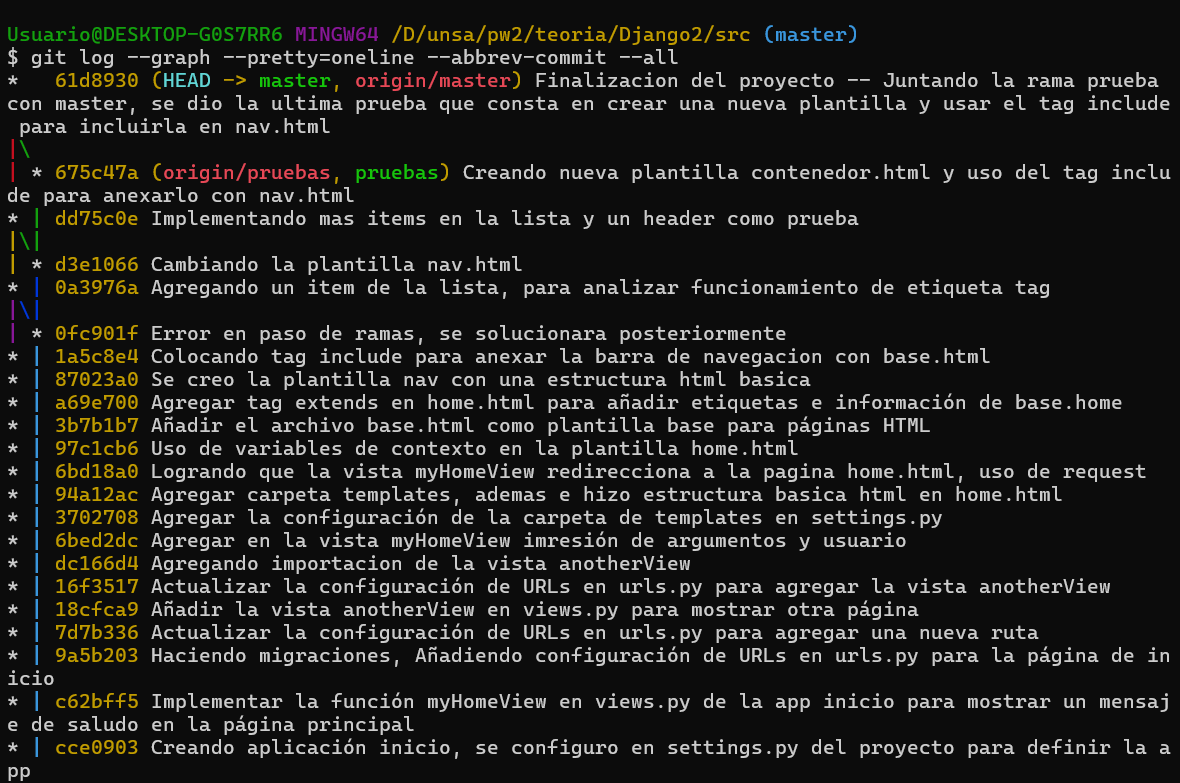
\includegraphics[width=1\textwidth, keepaspectratio]{img/commits1.png}
    \caption{Primera Parte commits}
  \end{figure}
  \newpage
  \begin{figure}[H]
    \centering
    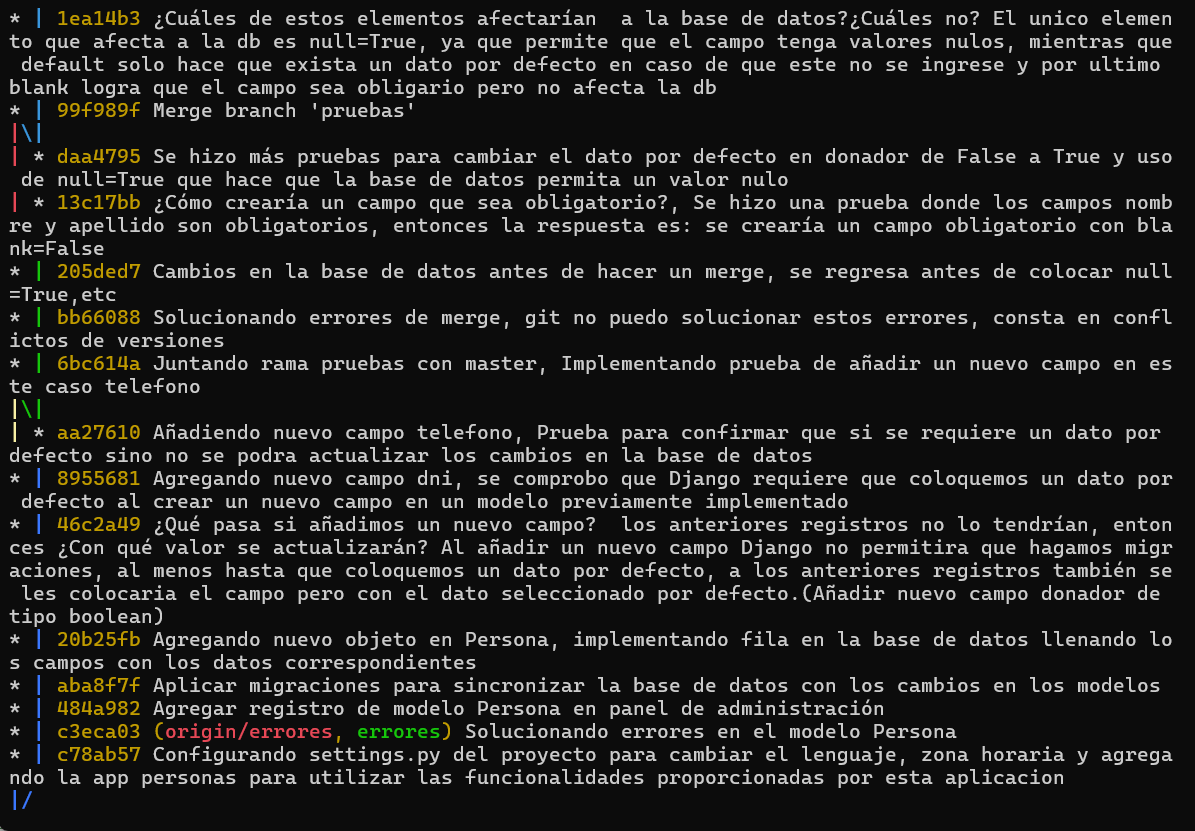
\includegraphics[width=1\textwidth, keepaspectratio]{img/commits2.png}
    \caption{Segunda Parte commits}
  \end{figure}
  \begin{figure}[H]
    \centering
    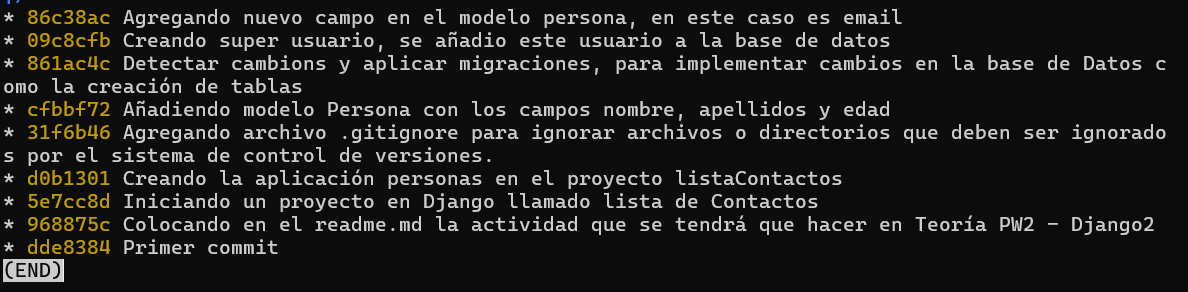
\includegraphics[width=1\textwidth, keepaspectratio]{img/commits3.png}
    \caption{Tercera Parte commits}
  \end{figure}

%%%%%%%%%%%%%%%%%%%%

  \section{URL de Repositorio Github}
  \begin{itemize}
    \item URL del Repositorio GitHub.
    \item \url{https://github.com/Victor-Gonzalo-Maldonado-Vilca/Django2.git}
  \end{itemize}
  \newpage

%%%%%%%%%%%%%%%%%%%%

  \section{Metodología}

%%%%%%%%%%%%
  
  \subsection{Creación del entorno de Trabajo}
  
%%%%%%

  \subsubsection{Carpeta de trabajo}
  \begin{lstlisting}[language=, caption={Creación del Directorio}]
    mkdir Django2 && cd Django2
  \end{lstlisting}
  
%%%%%%

  \subsubsection{Creación del Entorno Virtual}
  \begin{lstlisting}[language=, caption={Creación Entorno virtual}]
    virtualenv -p python3 .
  \end{lstlisting}
  
%%%%%%%

  \subsubsection{Activar entorno Virtual}
  \begin{lstlisting}[language=, caption={Activar Entorno Virtual}]
    Scripts/activate
  \end{lstlisting}
  
%%%%%%

  \subsubsection{Instalar Django en el entorno Virtual}
  \begin{lstlisting}[language=, caption={Instalar Django}]
    pip install Django
  \end{lstlisting}
  
%%%%%%

  \subsubsection{Creación carpeta del proyecto}
  \begin{lstlisting}[language=, caption={Carpeta src}]
    mkdir src && cd src
  \end{lstlisting}
  
%%%%%%

  \subsubsection{Inicializar git}
  \begin{lstlisting}[language=, caption={Comandos Iniciales}]
    echo "# Django2" >> README.md
    git init
    git add README.md
    git commit -m "Primer commit"
    git branch -M master
    git remote add origin https://github.com/Victor-Gonzalo-Maldonado-Vilca/Django2.git
    git push -u origin master
  \end{lstlisting}
  \newpage
  
%%%%%%

  \subsubsection{Uso de ramas}
  \textit{Se usarán las siguientes ramas: }
  \begin{lstlisting}
    git branch pruebas
    git branch errores
  \end{lstlisting}
  
%%%%%%

  \subsubsection{Crear .gitignore}
  Seguimos el siguiente Repositorio \url{https://github.com/django/django/blob/main/.gitignore}
  
%%%%%%%%%%%%
  
  \subsection{Creacion del proyecto y apps}
  
%%%%%%

  \subsubsection{Crear Proyecto}
  \begin{lstlisting}[language=, caption={Crear proyecto}]
    django-admin startproject listaContactos
  \end{lstlisting}
  
%%%%%%

  \subsubsection{Crear Apps}
  \begin{lstlisting}[language=, caption={Crear App}]
    python manage.py startapp personas
    python manage.py startapp inicio
  \end{lstlisting}
  
%%%%%%%%%%%%%%%%%%%%

  \section{Desarrollo del trabajo}
  \textit{Continuamos a partir del proyecto realizado en Django 1}
  
%%%%%%%%%%%%

  \subsection{Configuración settings.py del proyecto}
  
%%%%%%

  \subsubsection{Templates}
  \begin{figure}[H]
    \centering
    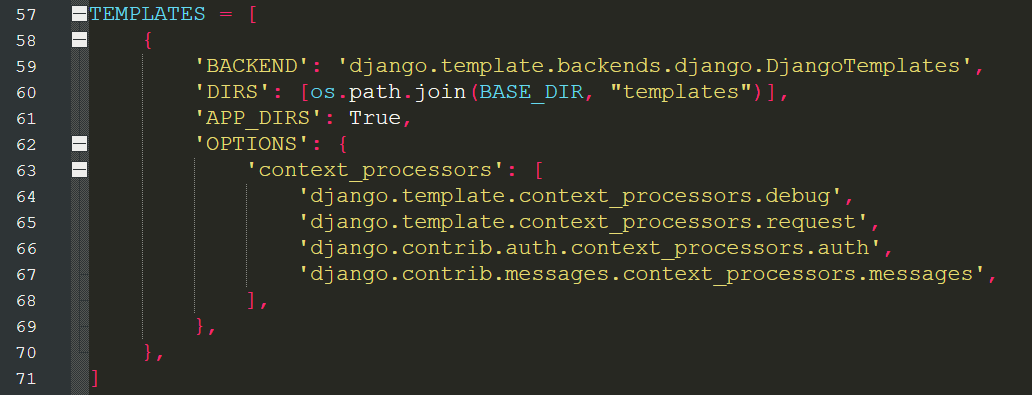
\includegraphics[width=1\textwidth, keepaspectratio]{img/templates.png}  
    \caption{Configuración de la carpeta templates}
  \end{figure}
  
%%%%%%

  \subsubsection{Install Apps}
  \begin{figure}[H]
    \centering
    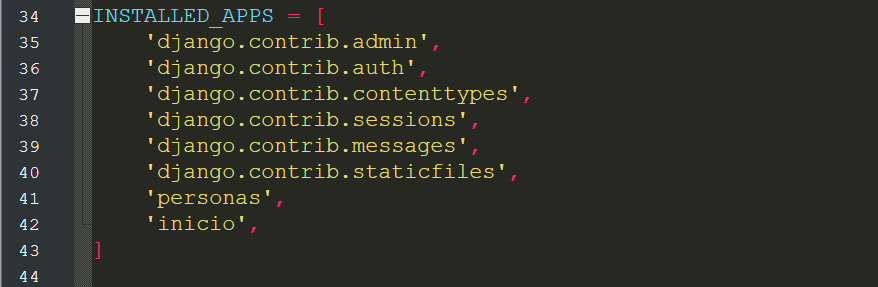
\includegraphics[width=1\textwidth, keepaspectratio]{img/inicio.png}  
    \caption{Definir aplicación inicio en el proyecto}
  \end{figure}
  
%%%%%%%%%%%%

  \subsection{Modelos -- Aplicación personas}
  El modelo \texttt{Persona} en Django define los atributos que se utilizarán para almacenar información sobre una persona en la base de datos. Cada atributo tiene un tipo de datos específico y ciertas reglas asociadas:
  \begin{itemize}
      \item \texttt{nombre}: Se trata de un campo de texto que puede almacenar hasta 100 caracteres y es obligatorio.
      \item \texttt{apellidos}: Otro campo de texto que también puede contener hasta 100 caracteres y debe ser completado.
      \item \texttt{edad}: Este campo guarda un número entero que representa la edad de la persona.
      \item \texttt{email}: Aquí se almacena la dirección de correo electrónico de la persona, con un límite de 100 caracteres.
      \item \texttt{donador}: Un campo booleano que indica si la persona es donante o no. Por defecto, se establece como \texttt{True} si no se especifica lo contrario.
      \item \texttt{dni}: Se utiliza para guardar el número de documento nacional de identidad (DNI) de la persona, aunque este campo puede quedar vacío si no se proporciona.
      \item \texttt{telefono}: Este campo guarda el número de teléfono de la persona y también puede quedar sin completar si no se desea proporcionar esta información.
  \end{itemize}
  Estos atributos permiten almacenar información relevante sobre una persona de manera organizada en la base de datos de la aplicación Django. Después se harán las migraciones 
  correspondientes.
  \begin{lstlisting}[language=Python, caption={Modelo Persona}]
    class Persona(models.Model):
      nombre    = models.CharField(max_length = 100, blank=False)
      apellidos = models.CharField(max_length = 100, blank=False)
      edad      = models.IntegerField()
      email     = models.CharField(max_length = 100)
      donador   = models.BooleanField(default=True)
      dni       = models.CharField(max_length = 8, null=True)
      telefono  = models.CharField(max_length = 9, null=True)
  \end{lstlisting}
  \newpage
  \begin{figure}[H]
    \centering
    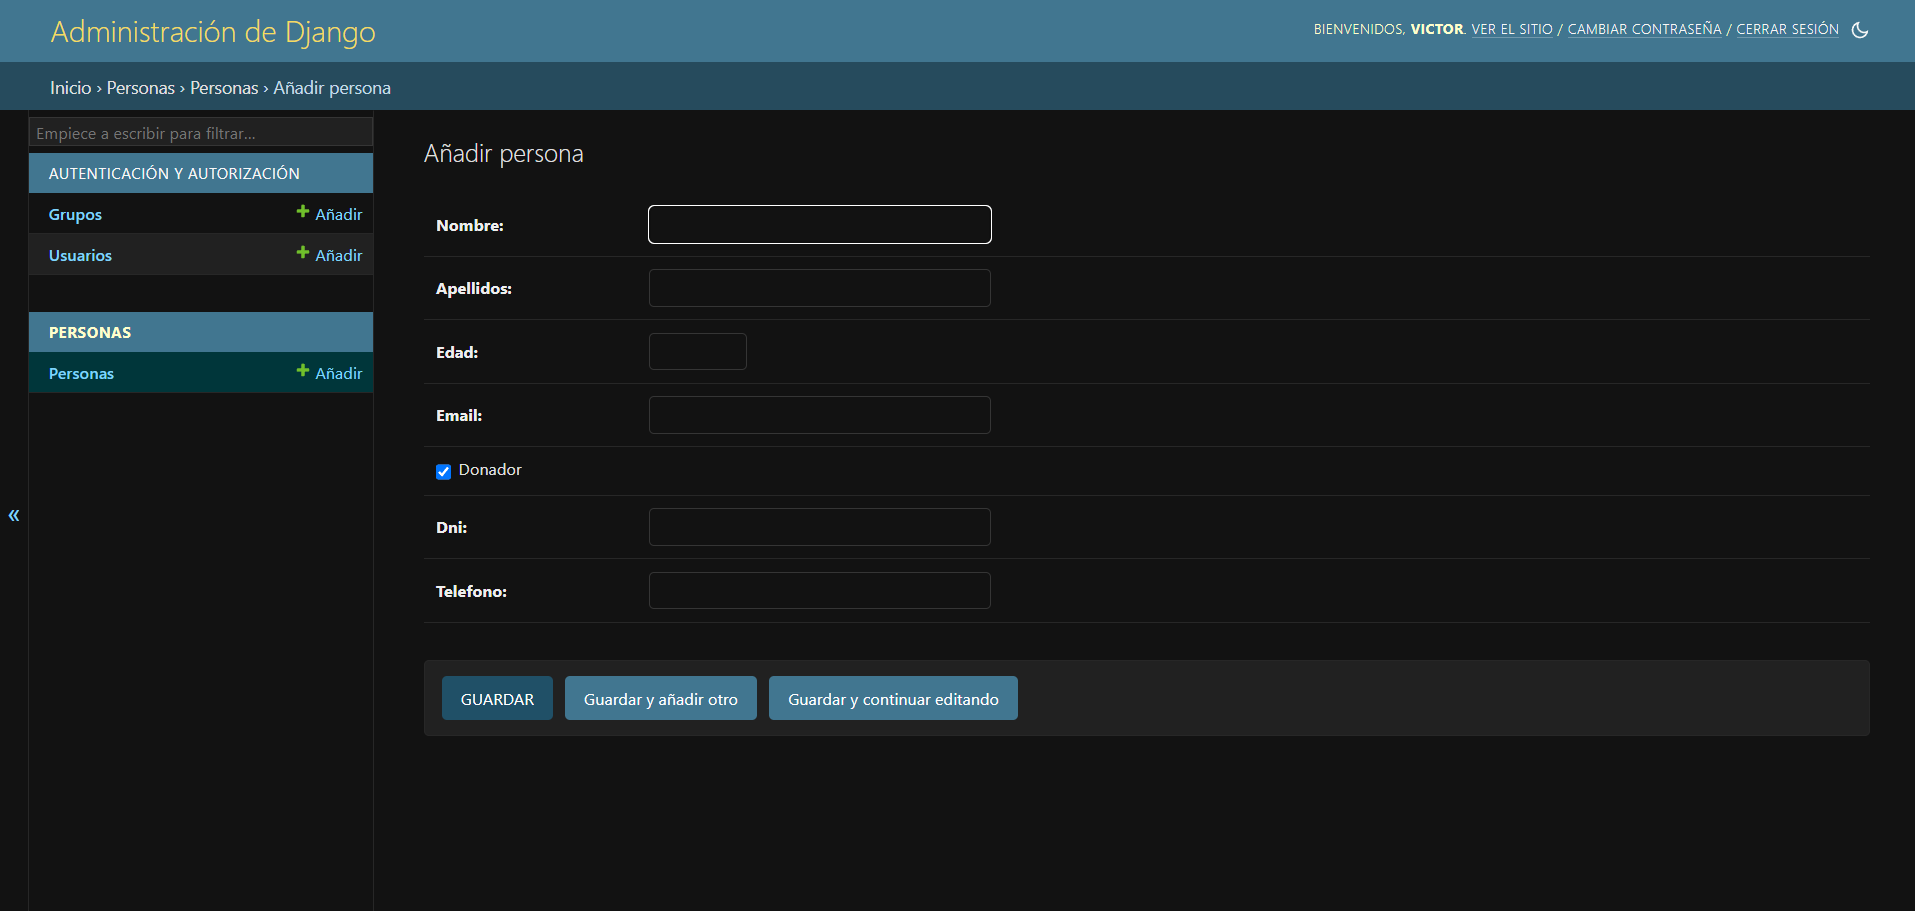
\includegraphics[width=1\textwidth, keepaspectratio]{img/model1.png}
    \caption{admin 1}
  \end{figure}
  \begin{figure}[H]
    \centering
    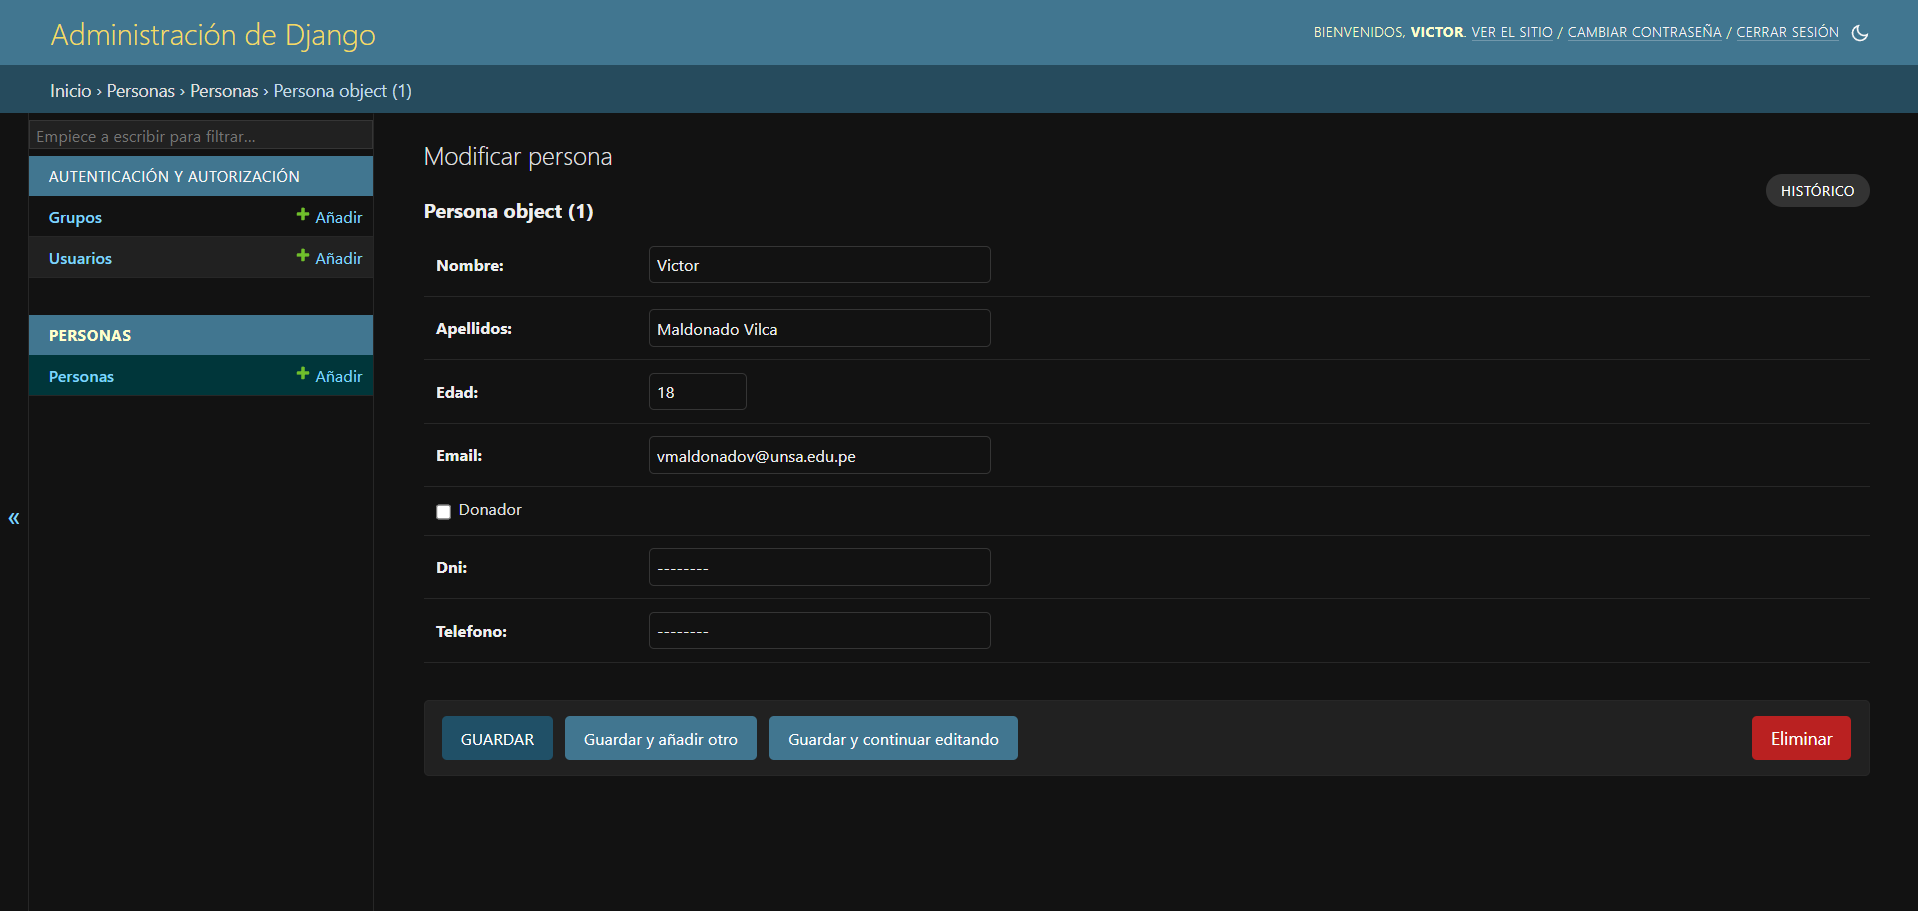
\includegraphics[width=1\textwidth, keepaspectratio]{img/model2.png}
    \caption{admin 2}
  \end{figure}
  \newpage
    
%%%%%%%%%%%%

  \subsection{Vistas -- Aplicación inicio}
  El archivo de vistas en Django define dos vistas importantes para la aplicación web. La primera vista, llamada \texttt{myHomeView}, 
  recibe un objeto \texttt{request} junto con argumentos adicionales, los cuales son impresos en la consola junto con el usuario 
  asociado a la solicitud. Esta vista luego renderiza una plantilla llamada \texttt{home.html}, proporcionando una respuesta HTML 
  basada en esta plantilla. La segunda vista, denominada \texttt{anotherView}, retorna una respuesta HTTP simple que contiene el 
  texto "Solo otra página". Estas vistas permiten manejar diferentes rutas en la aplicación y generar respuestas dinámicas basadas 
  en las solicitudes del usuario.
  \begin{lstlisting}[language=python]
    from django.shortcuts import render
    from django.http import HttpResponse

    # Create your views here.

    def myHomeView(request, *args, **kwargs):
        print(args, kwargs)
        print(request.user)
        return render(request, "home.html", {})
        
    def anotherView(request):
        return HttpResponse('<h1>Solo otra pagina</h1>')
  \end{lstlisting}

  
%%%%%%%%%%%%

  \subsection{URLs -- proyecto listaContactos}
  El archivo de configuración de URLs en Django, define las rutas URL que la aplicación web manejará. Este archivo importa 
  las vistas \texttt{myHomeView} y \texttt{anotherView} del módulo \texttt{inicio.views}, así como el módulo de administración 
  de Django. La lista \texttt{urlpatterns} contiene las rutas definidas para la aplicación: la ruta raíz que utiliza 
  \texttt{myHomeView} como la vista para la página de inicio, la ruta \texttt{another/} que utiliza \texttt{anotherView} 
  para mostrar una página adicional, y la ruta \texttt{admin/} que proporciona acceso a la interfaz de administración de 
  Django. Estas rutas permiten a la aplicación dirigir las solicitudes a las vistas correspondientes para generar las 
  respuestas adecuadas.

  \begin{lstlisting}[language=python]
    from django.contrib import admin
    from django.urls import path
    from inicio.views import myHomeView, anotherView

    urlpatterns = [
        path('', myHomeView, name='Pagina de Inicio'),
        path('another/', anotherView),
        path('admin/', admin.site.urls),
    ]
  \end{lstlisting}

  
%%%%%%%%%%%%%%%%%%%%%

  \section{Templates}
  
%%%%%%%%%%%%

  \subsection{Plantilla home.html}
  El siguiente código HTML define una plantilla base para una aplicación Django. Utiliza la sintaxis de plantillas 
  de Django para extender una plantilla base llamada \texttt{base.html}. Dentro del bloque de contenido definido por 
  \texttt 'block content', se inserta un mensaje "Hola Mundo desde Django" y "Con Templates" dentro 
  de las etiquetas h2 y h3, respectivamente. Adicionalmente, se muestra 
  el usuario actual con 'request.user' y su estado de autenticación.

  \begin{lstlisting}[language=html]
    <!DOCTYPE HTML>
    <html>
      <head>
        <title>Template Base</title>
      </head>
      <body>
        
        
        <h2>Hola Mundo desde Django</h2>
        <h3>Con Templates</h3>
        {{ request.user }}
        <br>
        {{ request.user.is_authenticated }}
        
      </body>
    </html>
  \end{lstlisting}
  
%%%%%%%%%%%%

  \subsection{Plantilla base.html}
  El siguiente código HTML define una plantilla base para una aplicación Django. La plantilla incluye el archivo 
  \texttt{nav.html} utilizando la sintaxis de inclusión de Django include 'nav.html'. Dentro del cuerpo de la página, 
  se muestra un encabezado de nivel 1 con el texto "Este es un texto de Base". Además, se define un bloque de contenido 
  utilizando la sintaxis de bloques de Django block content que inicialmente contiene el texto "Reemplazame". Este bloque 
  puede ser sobrescrito en plantillas que extiendan esta plantilla base.

  \begin{lstlisting}[language=html]
    <!DOCTYPE HTML>
    <html>
      <head>
        <title>Codigo para estudiantes desde Django</title>
      </head>
      <body>
        
        <h1> Este es un texto de Base</h1>
        
          Reemplazame
        
      </body>
    <html>
  \end{lstlisting}
  
%%%%%%%%%%%%

  \subsection{Plantilla nav.html}
  El siguiente código HTML define una estructura básica para una página web con un título y un menú de navegación. 
  En la sección \texttt{<head>}, se establece el título de la página como "Navegación". En el cuerpo de la página 
  (\texttt{<body>}), se incluye un elemento \texttt{<nav>} que contiene una lista desordenada (\texttt{<ul>})
  con varios elementos de lista (\texttt{<li>}) representando diferentes secciones de la página: Home, Primera, 
  Segunda, Tercera, Cuarta, Quinta y Sexta. Debajo del menú de navegación, se encuentra un encabezado de nivel 1 
  (\texttt{<h1>}) con el texto "Mi Página web usando Django". Finalmente, se incluye el contenido del archivo 
  \texttt{contenedor.html} utilizando la sintaxis de inclusión de Django 'include 'contenedor.html''.

  \begin{lstlisting}[language=html]
    <!DOCTYPE HTML>
    <html>
      <head>
        <title>Navegacion</title>
      </head>
      <body>
        <nav>
          <ul>
            <li>Home</li>
            <li>Primera</li>
            <li>Segunda</li>
            <li>Tercera</li>
            <li>Cuarta</li>
            <li>Quinta</li>
            <li>Sexta</li>
          </ul>
        </nav>
        <h1>Mi Pagina web usando Django</h1>
        
      </body>
    </html>
  \end{lstlisting}

%%%%%%%%%%%%

  \subsection{Plantilla contenedor.html}
  El siguiente código HTML define una estructura simple de una página web que incluye un contenedor de contenido. 
  En la sección \texttt{<head>}, se establece el título de la página como "Contenedor". En el cuerpo de la página 
  (\texttt{<body>}), se encuentra un elemento \texttt{<div>} que contiene dos encabezados. El primer encabezado es de 
  nivel 2 (\texttt{<h2>}) con el texto "Hola Mundo", y el segundo es de nivel 3 (\texttt{<h3>}) con el texto "DJANGO".

  \begin{lstlisting}[language=html]
    <!DOCTYPE HTML>
    <html>
      <head>
        <title>Contenedor</title>
      </head>
      <body>
        <div>
          <h2>Hola Mundo</h2>
          <h3>DJANGO</h3>
        </div>
      </body>
    </html>
  \end{lstlisting}
  
  
%%%%%%%%%%%%

  \subsection{Ejecución del servidor}
  Este siguiente comando inicia el servidor local de Django. Una vez ejecutado, el servidor estará disponible por defecto en la dirección 
  \texttt{http://127.0.0.1:8000/}. Desde esta dirección, se puede acceder a las diferentes vistas y funcionalidades del 
  proyecto Django.
  \begin{lstlisting}[language=bash]
    python manage.py runserver
  \end{lstlisting}
  \begin{figure}[H]
    \centering
    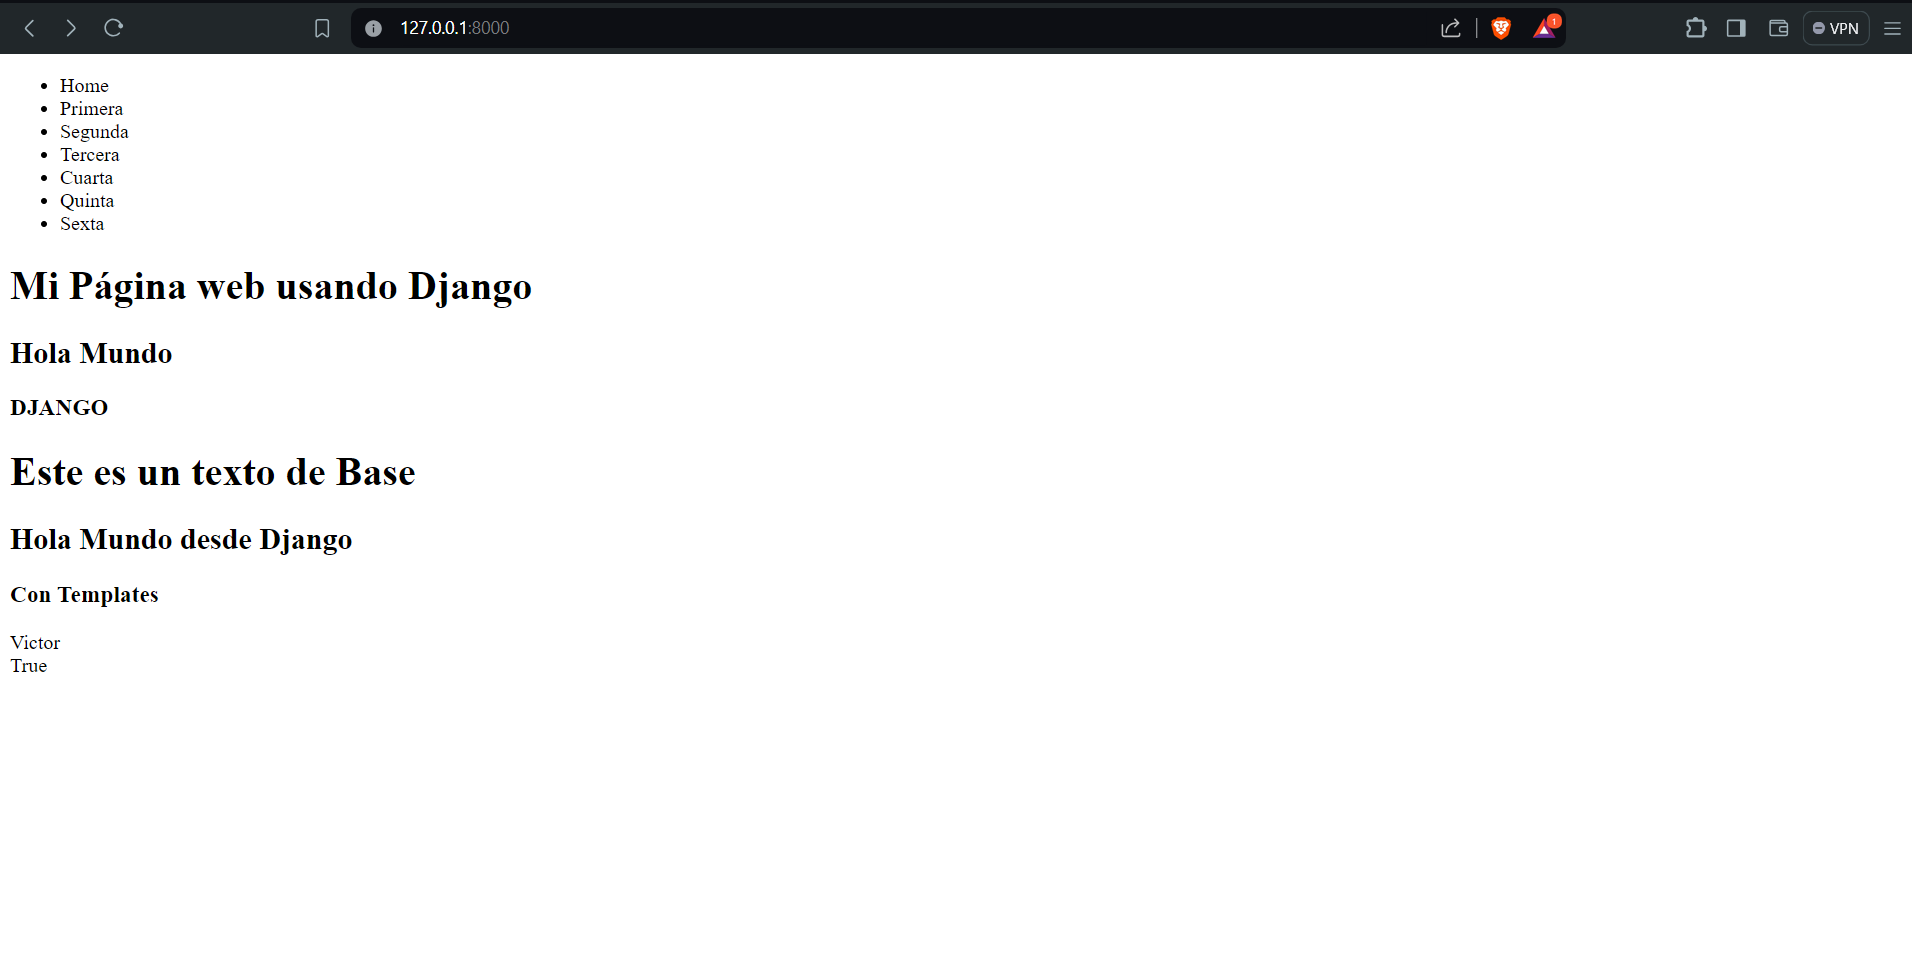
\includegraphics[width=1\textwidth, keepaspectratio]{img/ejecucion1.png}
    \caption{Path ''}
  \end{figure}
  \begin{figure}[H]
    \centering
    
\includegraphics[width=1\textwidth, keepaspectratio]{img/ejecucion2.png}
    \caption{Path 'another/'}
  \end{figure}


%%%%%%%%%%%%%%%%%%%%
	
  \subsection{Uso de GitHub}
  
%%%%%%%%%%%%%%%%%%%%

	\subsubsection{Usuario de GitHub}
  \begin{figure}[H]
    \centering
    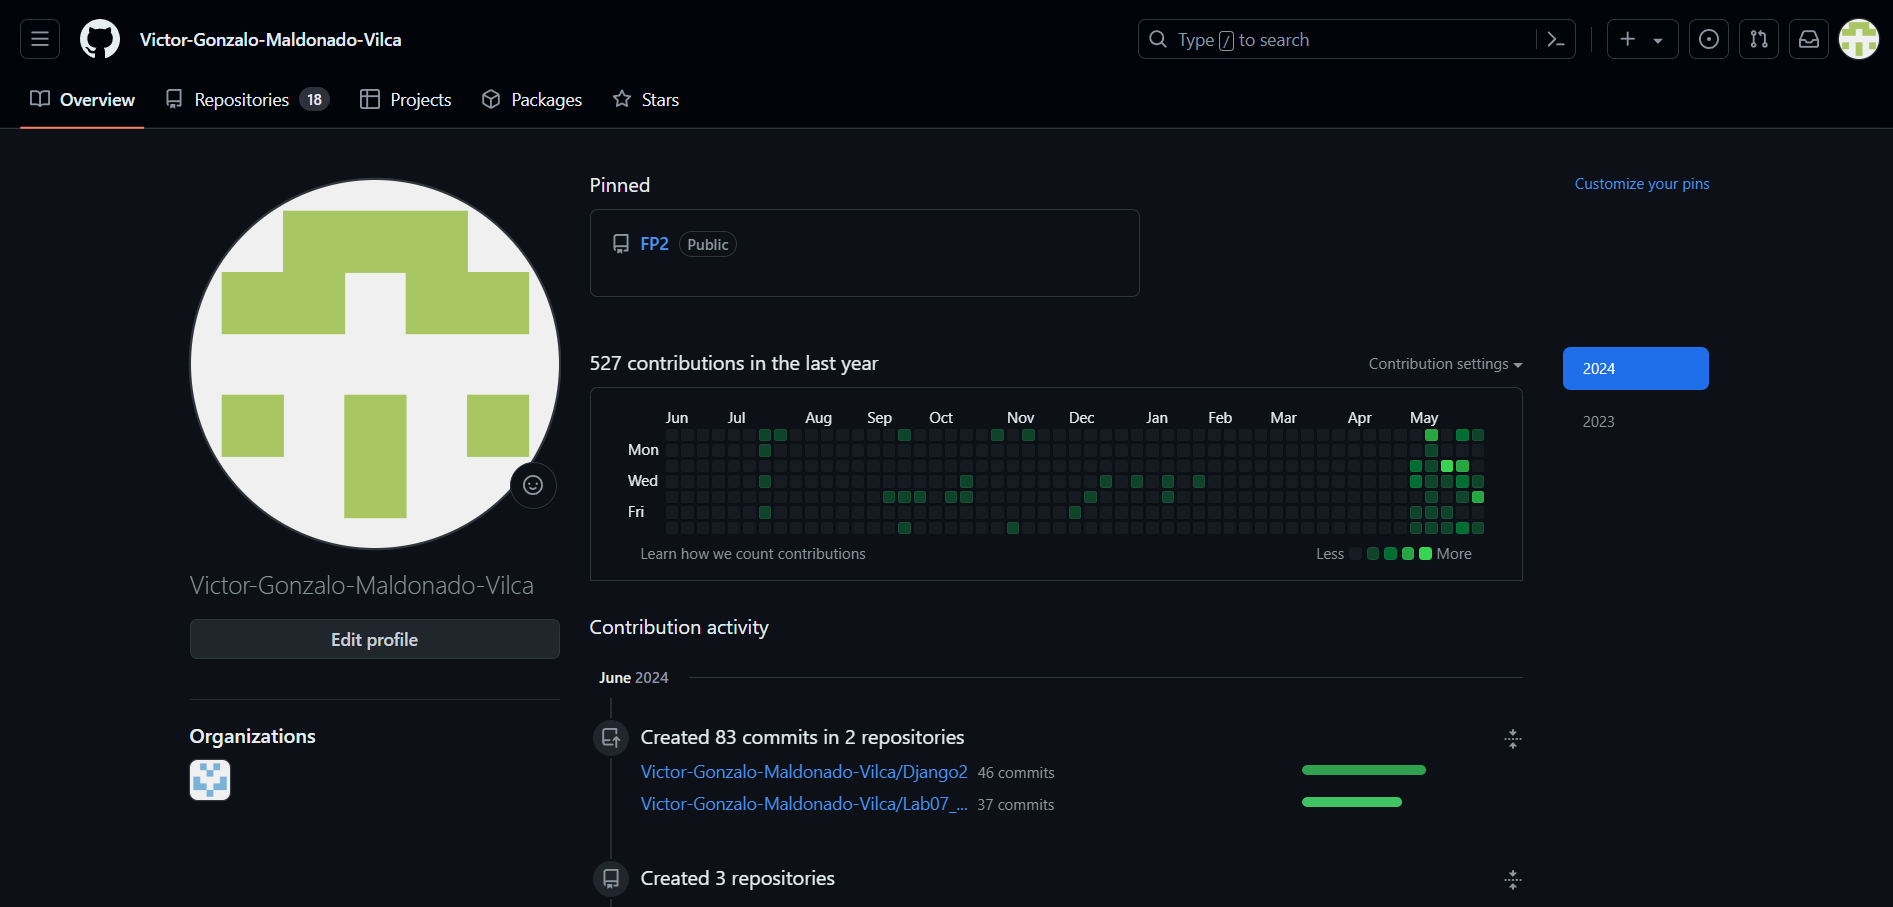
\includegraphics[width=1\textwidth, keepaspectratio]{img/usuario.png}
    \caption{Usuario}
  \end{figure}
  
%%%%%%%%%%%%%%%%%%%%

  \subsubsection{Creación de un Nuevo Repositorio}
  \begin{figure}[H]
    \centering
    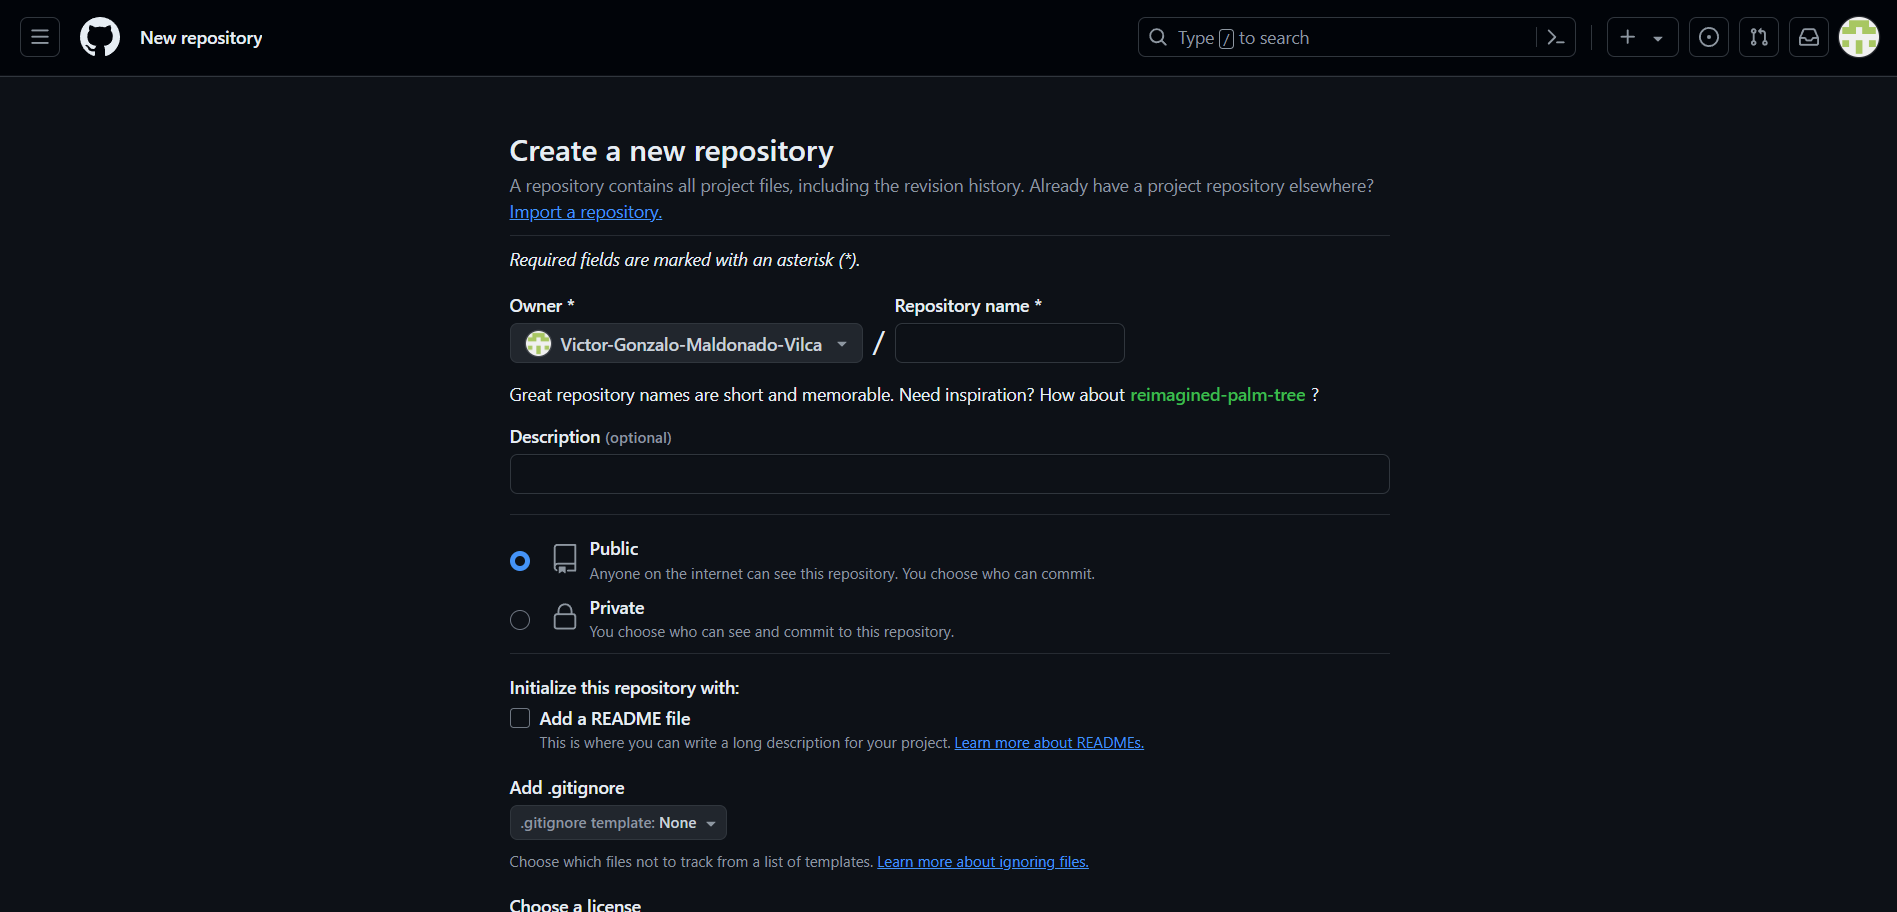
\includegraphics[width=1\textwidth, keepaspectratio]{img/crearRepo.png}
    \caption{Crear Repositorio}
  \end{figure}
  
  
%%%%%%%%%%%%%%%%%%%%  
  
  \subsubsection{Implementación de Readme.md}
  \begin{figure}[H]
    \centering
    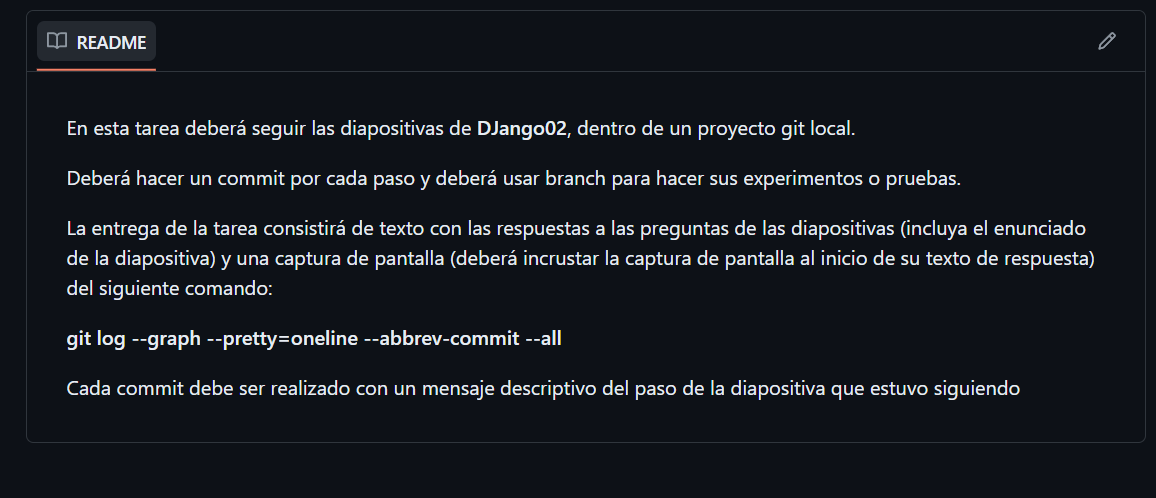
\includegraphics[width=1\textwidth, keepaspectratio]{img/readme.png}
    \caption{README.md}
  \end{figure}
  
%%%%%%%%%%%%%%%%%%%%

	\subsubsection{Registro de cambios en mi código}
  \begin{figure}[H]
    \centering
    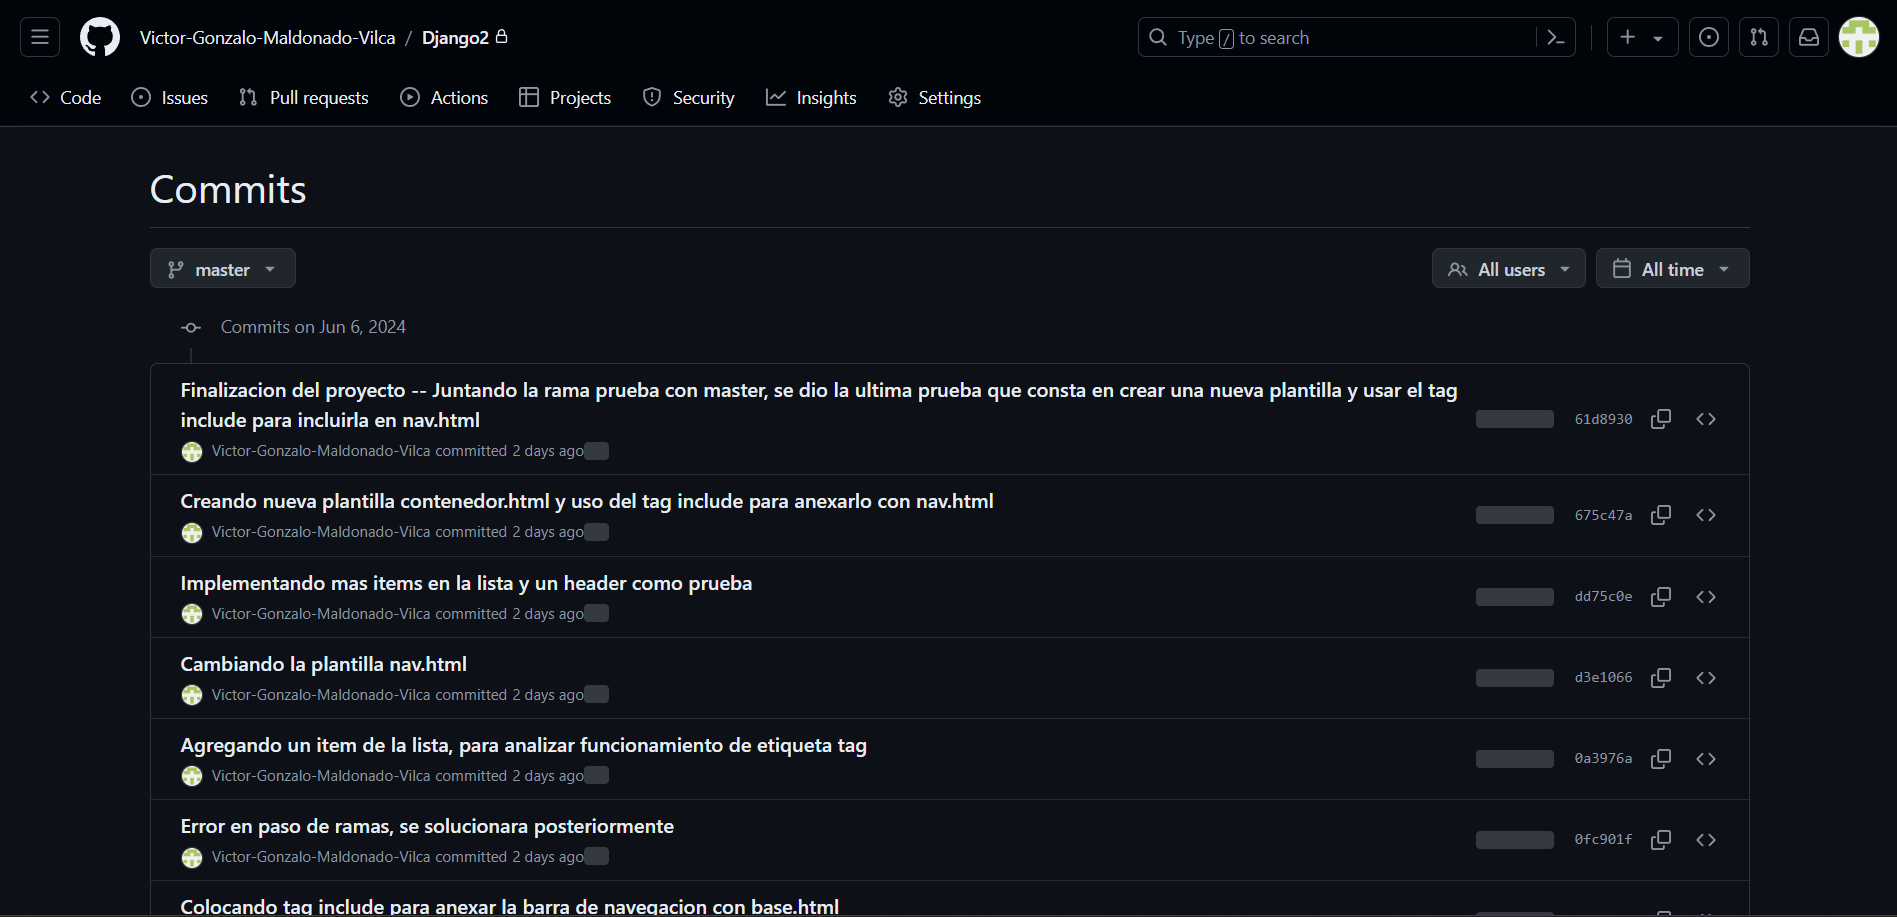
\includegraphics[width=1\textwidth, keepaspectratio]{img/commit.png}
    \caption{Commits}
  \end{figure}
  
%%%%%%%%%%%%%%%%%%%%

	\subsubsection{Uso de Ramas}
  \begin{figure}[H]
    \centering
    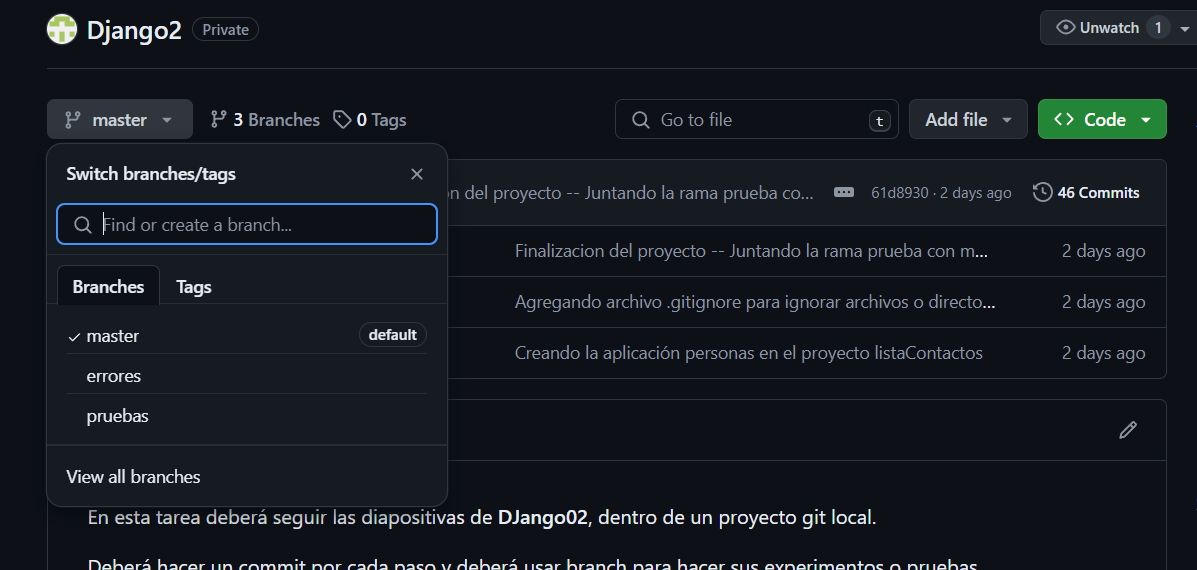
\includegraphics[width=1\textwidth, keepaspectratio]{img/ramas.png}
    \caption{Ramas}
  \end{figure}
	
%%%%%%%%%%%%%%%%%%%%

	\subsubsection{Repositorio}
  \begin{figure}[H]
    \centering
    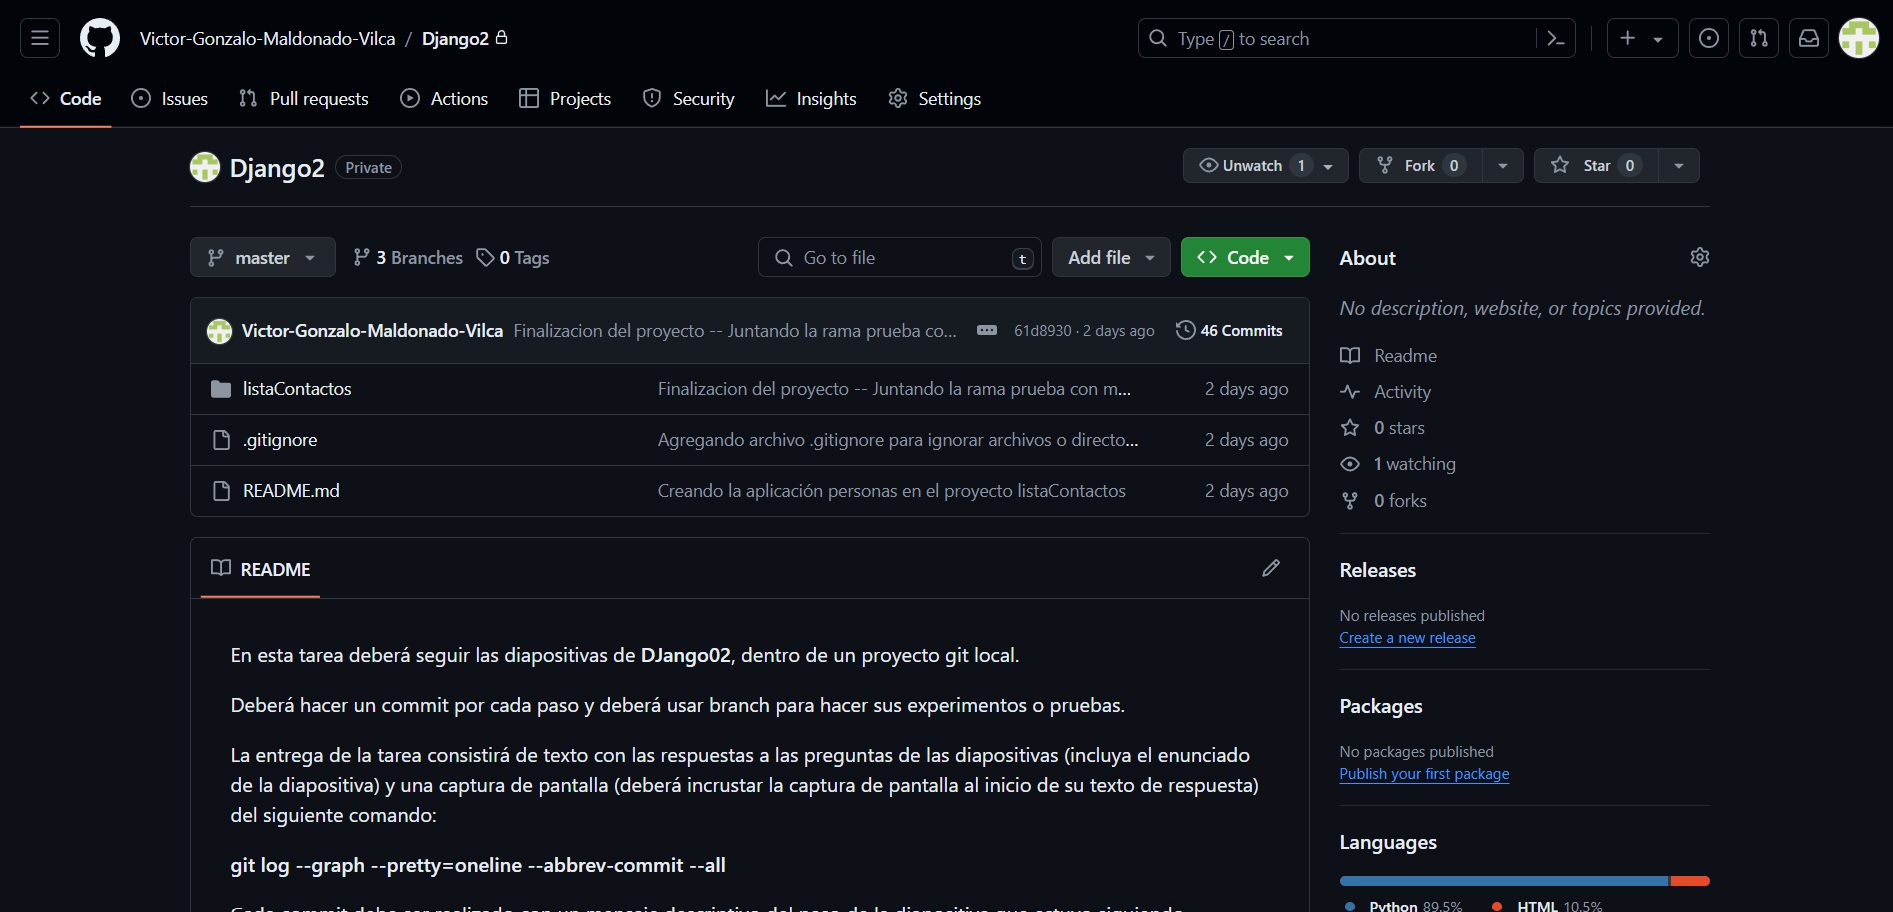
\includegraphics[width=1\textwidth, keepaspectratio]{img/repositorio.png}
    \caption{Repositorio}
  \end{figure}
  
%%%%%%%%%%%%%%%%%%%%

	\subsubsection{Proyecto compartido con el profesor de github}
  \begin{figure}[H]
    \centering
    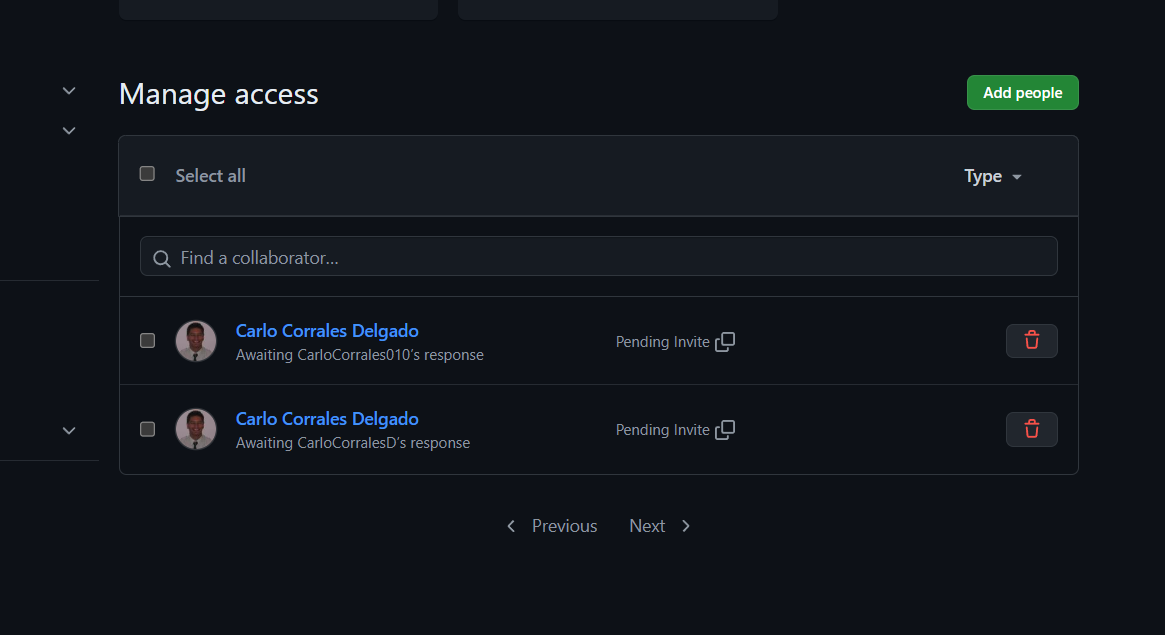
\includegraphics[width=1\textwidth, keepaspectratio]{img/compartir.png}
    \caption{Compartir con el Docente}
  \end{figure}
  
%%%%%%%%%%%%%%%%%%%%

  \section{Recomensaciones}
  \begin{itemize}
    \item Seguir las mejores prácticas de desarrollo de Django, como la separación de la lógica de negocios en vistas y 
    la creación de plantillas reutilizables.
    \item Realizar pruebas unitarias y de integración para garantizar la calidad del código, y asegúrate de implementar 
    medidas de seguridad en tu aplicación.
  \end{itemize}

%%%%%%%%%%%%%%%%%%%%

  \section{Conclusiones}
  \begin{itemize}
    \item La utilización de herramientas como el servidor de desarrollo de Django y el sistema de plantillas facilitaron 
    el desarrollo ágil y eficiente de la aplicación.
    \item Django es un framework web potente y versátil que permite desarrollar aplicaciones web de manera rápida y eficiente.
    \item La arquitectura MVC (Modelo-Vista-Controlador) de Django ayuda a organizar el código de manera estructurada y modular, 
    lo que facilita la mantenibilidad y escalabilidad de las aplicaciones.
    \item Con un buen entendimiento de Django y siguiendo las mejores prácticas de desarrollo, se pueden crear aplicaciones web 
    robustas y de alto rendimiento.
  \end{itemize}
  
%%%%%%%%%%%%%%%%%%%%
	\newpage
	\subsection{\textcolor{red}{Rúbrica para el contenido del Informe y demostración}}
	\begin{itemize}			
		\item El alumno debe marcar o dejar en blanco en celdas de la columna \textbf{Checklist} si cumplio con el ítem correspondiente.
		\item Si un alumno supera la fecha de entrega,  su calificación será sobre la nota mínima aprobada, siempre y cuando cumpla con todos lo items.
		\item El alumno debe autocalificarse en la columna \textbf{Estudiante} de acuerdo a la siguiente tabla:
	
		\begin{table}[ht]
			\caption{Niveles de desempeño}
			\begin{center}
			\begin{tabular}{ccccc}
    			\hline
    			 & \multicolumn{4}{c}{Nivel}\\
    			\cline{1-5}
    			\textbf{Puntos} & Insatisfactorio 25\%& En Proceso 50\% & Satisfactorio 75\% & Sobresaliente 100\%\\
    			\textbf{2.0}&0.5&1.0&1.5&2.0\\
    			\textbf{4.0}&1.0&2.0&3.0&4.0\\
    		\hline
			\end{tabular}
		\end{center}
	\end{table}	
	

	\end{itemize}

 
	
	\begin{table}[H]
		\caption{Rúbrica para contenido del Informe y demostración}
		\setlength{\tabcolsep}{0.5em} % for the horizontal padding
		{\renewcommand{\arraystretch}{1.5}% for the vertical padding
		%\begin{center}
		\begin{tabular}{|p{2.7cm}|p{7cm}|x{1.3cm}|p{1.2cm}|p{1.5cm}|p{1.1cm}|}
			\hline
    		\multicolumn{2}{|c|}{Contenido y demostración} & Puntos & Checklist & Estudiante & Profesor\\
			\hline
			\textbf{1. GitHub} & Hay enlace URL activo del directorio para el  laboratorio hacia su repositorio GitHub con código fuente terminado y fácil de revisar. &2 &X &2 & \\ 
			\hline
			\textbf{2. Commits} &  Hay capturas de pantalla de los commits más importantes con sus explicaciones detalladas. (El profesor puede preguntar para refrendar calificación). &4 &X &4 & \\ 
			\hline 
			\textbf{3. Código fuente} &  Hay porciones de código fuente importantes con numeración y explicaciones detalladas de sus funciones. &2 &X &2 & \\ 
			\hline 
			\textbf{4. Ejecución} & Se incluyen ejecuciones/pruebas del código fuente  explicadas gradualmente. &2 &X &2 & \\ 
			\hline			
			\textbf{5. Pregunta} & Se responde con completitud a la pregunta formulada en la tarea.  (El profesor puede preguntar para refrendar calificación).  &2 &X &2 & \\ 
			\hline	
			\textbf{6. Fechas} & Las fechas de modificación del código fuente estan dentro de los plazos de fecha de entrega establecidos. &2 &X &2 & \\ 
			\hline 
			\textbf{7. Ortografía} & El documento no muestra errores ortográficos. &2 &X &2 & \\ 
			\hline 
			\textbf{8. Madurez} & El Informe muestra de manera general una evolución de la madurez del código fuente,  explicaciones puntuales pero precisas y un acabado impecable.   (El profesor puede preguntar para refrendar calificación).  &4 &X &4 & \\ 
			\hline
			\multicolumn{2}{|c|}{\textbf{Total}} &20 & &20 & \\ 
			\hline
		\end{tabular}
		%\end{center}
		%\label{tab:multicol}
		}
	\end{table}


%%%%%%%%%%%%%%%%%%%%%%%%%%%%%%%%%%%%%%%%%%%%%%%%%%%%%%%%%%%%%%%%%%%
	
  \newpage
  \section{Referencias}
  \begin{itemize}
    \item \url{https://docs.djangoproject.com/en/5.0/}
    \item \url{https://docs.github.com/es}
    \item \url{https://git-scm.com/doc}
  \end{itemize}
  
%%%%%%%%%%%%%%%%%%%% 
%\clearpage
%\bibliographystyle{apalike}
%\bibliographystyle{IEEEtranN}
%\bibliography{bibliography}
			
\end{document}
